\documentclass{article}
\usepackage{enumitem}
\usepackage{lipsum} 
\usepackage{geometry} 
\usepackage{booktabs}
\usepackage{tabularx}
\usepackage{graphicx}
\usepackage{setspace}
\usepackage{xcolor}
\usepackage{colortbl}
\usepackage{caption}
\usepackage{hyperref}
\geometry{
    top=1in,
    bottom=1in,
    left=1in,
    right=1in,
}
\begin{document}
\section*{ \Huge General Introduction}\vspace{0.5cm} 
\setstretch{1.5}
\hspace{1.5em}Leaving home for college or a new adventure is a big step towards independence whether you're a Tunisian student far from family or just living on your own for the first time, it's an exciting but challenging time, especially when it comes to cooking being away from home can leave you feeling a bit lost, especially if you're not sure how to cook.\vspace{0.2cm} \\ 
%\hspace{1.5em}
That's where "Taste \& Share" comes in! we understand the struggles of being alone and away from the comfort of home, which is why we've gathered simple and healthy recipes to make cooking easier for you as a student, you're often juggling classes, assignments, and social activities, leaving little time and energy for cooking elaborate meals we get it you need meals that are quick, affordable, and nutritious, so you can stay focused and energized throughout the day , our platform is designed with your needs in mind, offering a variety of easy-to-follow recipes that can be prepared with minimal ingredients and time plus, by cooking at home instead of constantly ordering takeout or dining out, you can save money in the long run while also enjoying healthier meals.\vspace{0.2cm}\\ We know that living away from home can sometimes leave you feeling homesick and longing for familiar flavors, that's why our platform offers a diverse array of recipes to suit every palate and culinary skill level. From simple one-pot wonders to comforting dishes that remind you of home-cooked meals, we've got something for everyone.\vspace{0.2cm}\\And with our friendly community of fellow students and food enthusiasts, you can connect with others who are going through the same experience as you. You can find, save, and share recipes with friends easily, making the cooking experience even more enjoyable. So whether you're craving a taste of home or ready to try something new, "Taste \& Share" is here to make your cooking journey fun, delicious, and budget-friendly, wherever you are.
\vspace{0.2cm}\\In our project, we implemented Scrum, an agile framework for managing work. Scrum breaks down tasks into short sprints, typically lasting one to four weeks, fostering collaboration and adaptability. With daily stand-up meetings, sprint planning, reviews, and retrospectives, Scrum promotes transparency and continuous improvement, enabling teams to deliver value more efficiently.
\newpage
\section*{\Huge CHAPTER 1\vspace{0.5cm}\\Requirements Specification}
\vspace{1.5cm}

{\Large \textbf{1.1\hspace{1em}Introduction}}\vspace{0.2cm}
\\In this part of our chapter, we'll dig into the details of what our project needs. This means figuring out what it should do (functional requirements), how it should perform (non-functional requirements), and who will use it (actors). Then, we'll create a simple diagram (the global use case diagram) to show how everything fits together. This diagram will help us understand how different parts of our project interact. Finally, we'll talk about our backlog product along with our work environment(Project Management Methodology/Software environment), which is a list of tasks and features we need to prioritize. By doing all this, we'll make sure we're on track to meet our project's goals.\vspace{0.5cm}
\\{\Large \textbf{1.2\hspace{1em}Requirements Identification}}\vspace{0.2cm}
\\The requirements specification is crucial for building a product. It outlines how the system should work and any limitations on its design. By establishing these guidelines upfront, we ensure that the development team creates a product that meets the customers' needs. Functional requirements describe what the system should do, while non-functional requirements focus on how it should perform. Together, these requirements provide a clear roadmap for product development, ensuring that the end result aligns with customer expectations and functions effectively.\vspace{0.5cm}
\\{\large \textbf{1.2.1\hspace{1em}Functional requirements}}\vspace{0.2cm}
\\Functional requirements, often referred to as the functional specification, serve as a comprehensive set of guidelines detailing the primary objectives of the system and how it serves its users. These requirements highlight the core functionalities that the development team needs to implement throughout the development process. By clearly defining what the system must accomplish, functional requirements enable the team to monitor their progress effectively and ensure that they're on track to meet the project's goals.\vspace{0.1cm}
\begin{itemize}[label=$\bullet$]
	\item Authenticate
	\item Consult Recipes
	\item Give Opinions
	\item Contact Other Users
\newpage
\noindent
CHAPTER 1.  REQUIREMENTS SPECIFICATION \\
\underline{\hspace{\textwidth}} \vspace{0.1cm}
	\item Manage Recipes	
	\item Manage Users
	\item Manage Comments 
	\item Manage Categories
\end{itemize}
\vspace{0.5cm}
{\large \textbf{1.2.2\hspace{1em}Non-Functional requirements}}
\vspace{0.2cm}
\\Non-functional requirements, in contrast to functional ones, delineate the various attributes and characteristics of the developed system while it executes its use cases. They primarily focus on aspects such as security, portability, usability, and more, essentially setting the standards for how well the functional requirements should be met. These requirements are critical as they ensure that the system operates within predefined parameters and meets user expectations regarding performance and quality. Although the system may technically still function without adhering strictly to non-functional requirements, it would likely fall short in meeting the overall needs and desires of both the owner and the end-user. Thus, it is imperative to prioritize and fulfill these requirements to deliver a successful and satisfactory product.\vspace{0.1cm}
\begin{itemize}[label=$\bullet$]
	\item Security and Safety :\vspace{0.1cm}
\\- The app must encrypt user's password and ensure the Security of his account with MFA.
\\- The app should ensure user's Safety by blocking sensitive contents and ban suspiscious users.
	\item Easy to use : \vspace{0.1cm}
\\- The app should provide usability for everybody regardless his knowledge in technology.
\\- Provide a tutorial for who use the app for the first time.
	\item Maintainable\vspace{0.1cm}
\\- The app should runs smoothly.
\\- The app should remain reliable and functions effectively.
	\item Availability\vspace{0.1cm}
\\- The app should be accessible to everyone.
\\- The app should be available  24/7 to users.
\end{itemize}
\newpage
\noindent
CHAPTER 1.  REQUIREMENTS SPECIFICATION \\
\underline{\hspace{\textwidth}} \vspace{0.2cm}\\
{\large \textbf{1.2.3\hspace{1em}Actors Identification}}\vspace{0.2cm}
\\An actor embodies a user's role when interacting with the system. They represent different user personas and their specific interactions with the system's functionalities, guiding its behavior. Identifying these actors helps tailor the system to meet diverse user needs effectively.\vspace{0.8cm}
\begin{table}[h]
    \centering
    \begin{tabularx}{\textwidth}{X|X}
        \toprule
        \textbf{\color{blue!70} Actors} & \textbf{\color{blue!70} Roles} \\ 
        \midrule
        Administrator &  \begin{itemize}[label=$\bullet$]
	\item Authenticate
	\item Manage Recipes	
	\item Manage Users
	\item Manage Comments 
	\item Manage Categories
\end{itemize} \\
        \midrule
        User & \begin{itemize}[label=$\bullet$]
	\item Authenticate
	\item Consult Recipes
	\item Give Opinions
	\item Contact Other Users
\end{itemize}\\
        \bottomrule
    \end{tabularx}
    \caption{Detailed description of the actors}
    \label{tab:actors_roles}
\end{table}
\newpage
\noindent
CHAPTER 1.  REQUIREMENTS SPECIFICATION \\
\underline{\hspace{\textwidth}} \vspace{0.2cm}\\
{\Large \textbf{1.3\hspace{1em}Global use case diagram}}\vspace{0.2cm}
\\The following figure showcases the global use case diagram of our project.\vspace{0.2cm}
\begin{figure}[h]
    \centering
    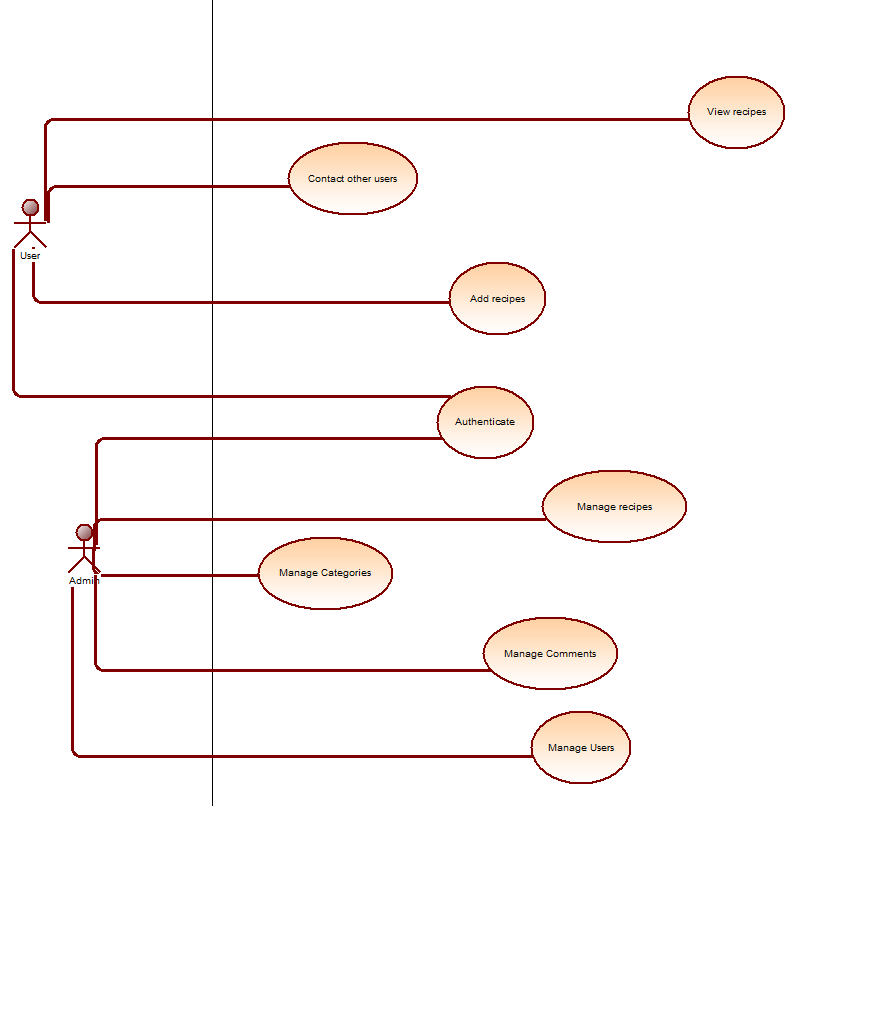
\includegraphics[width=0.8\textwidth,height=0.9\textheight,keepaspectratio]{use case dia}
    \caption{global use case diagram}
    \label{fig:example}
\end{figure}
\newpage
\noindent
CHAPTER 1.  REQUIREMENTS SPECIFICATION \\
\underline{\hspace{\textwidth}} \vspace{0.2cm}\\
{\Large \textbf{1.4\hspace{1em}Product backlog}}\vspace{0.2cm}
\\The backlog product is a prioritized list of tasks essential for developing the project, structured according to the levels necessary to meet system requirements. This hierarchical organization ensures that the most critical tasks are placed at the top level, enabling the development team to identify and focus on delivering them first. By following this approach, the team can streamline their efforts, ensuring that the project progresses in alignment with the system's overarching goals and priorities.\vspace{0.8cm}
\begin{table}[h]
    \centering
    \begin{tabularx}{\textwidth}{lX@{\hspace{1em}}c@{\hspace{7em}}c} 
        \toprule
        \textbf{\color{blue!70} User Story} & \textbf{\color{blue!70} Priority} & \textbf{\color{blue!70} Sprint} & \textbf{\color{blue!70} Estimation} \\ 
        \midrule
        As a user, I can authenticate & 1 & 0 & Medium \\
        \midrule
        As a User, I can add recipes & 1 & 0 & Medium \\
        \midrule
        As an admin, I can manage categories & 1 & 0 & Medium \\
        \midrule
        As a user, I can contact other users & 2 & 1 & High \\
        \midrule
        As a User I can view recipes & 2 & 1& Medium \\
        \midrule
        As an admin, I can manage users & 2 & 1 & High \\
        \bottomrule
    \end{tabularx}
    \caption{Product backlog}
    \label{tab:user_stories}
\end{table}

\newpage
\noindent
CHAPTER 1.  REQUIREMENTS SPECIFICATION \\
\underline{\hspace{\textwidth}} \vspace{0.2cm}\\
{\Large \textbf{1.5\hspace{1em}Work environment}}\vspace{0.2cm}\\
In pursuit of our project goals, we've embraced the Agile methodology, specifically Scrum, along with employing various software tools. This approach allows us to adapt quickly to changing requirements, collaborate effectively as a team, and deliver high-quality results efficiently. By leveraging Agile principles and utilizing the right software, we're confident in our ability to achieve our objectives with flexibility and innovation.\vspace{0.2cm}\\
{\large \textbf{1.5.1\hspace{1em}Project Management Methodology}}
\\Scrum is a form of agile project management. You can think of it more like a framework than as a project management methodology in itself.
With Scrum, work is split into short cycles known as “sprints”, which usually last about 1-2 weeks. Work is taken from the backlog for each sprint iteration,
Small teams are led by a Scrum Master (who is not the same as the project manager) for the duration of the sprint, after which they review their performance in a “sprint retrospective” and make any necessary changes before starting the next sprint.
\\
\vspace{0.3cm}
\begin{figure}[htbp]
    \centering
    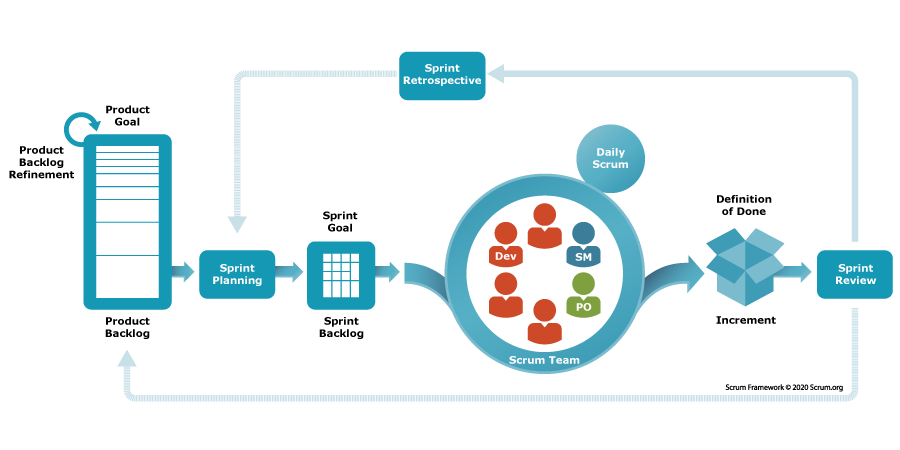
\includegraphics[width=1\textwidth]{1234}
    \caption{An iteration according to the Scrum method}
    \label{fig:design2}
\end{figure}
\newpage
\noindent
CHAPTER 1.  REQUIREMENTS SPECIFICATION \\
\underline{\hspace{\textwidth}} \vspace{0.2cm}\\
{\large \textbf{1.5.2\hspace{1em}Software environment}}\vspace{0.2cm}
\begin{figure}[htbp]
    \centering
    
\includegraphics[width=0.15\textwidth]{ddd}
    \caption{Visual Studio Code}
    \label{fig:design1}
\end{figure}

\paragraph{Visual Studio Code :} 
Visual Studio Code is a lightweight but powerful source code editor which runs on your desktop and is available for Windows, macOS and Linux. It comes with built-in support for JavaScript, TypeScript and Node.js and has a rich ecosystem of extensions for other languages and runtimes (such as C++, C\#, Java, Python, PHP, Go, .NET)(microsoft)

\vspace{1cm}

\begin{figure}[htbp]
    \centering
    
\includegraphics[width=0.2\textwidth]{eee}
    \caption{PHP}
    \label{fig:design2}
\end{figure}

\paragraph{PHP :} 
(recursive acronym for PHP: Hypertext Preprocessor ) is a widely-used open source general-purpose scripting language that is especially suited for web development and can be embedded into HTML(PHP documentation)
\vspace{1cm}
\newpage
\noindent
CHAPTER 1.  REQUIREMENTS SPECIFICATION \\
\underline{\hspace{\textwidth}} \vspace{0.2cm}\\
\begin{figure}[htbp]
    \centering
    
\includegraphics[width=0.2\textwidth]{ccc}
    \caption{Angular}
    \label{fig:design3}
\end{figure}
\paragraph{Angular :} 
is a TypeScript-based open-source web application framework primarily maintained by Google and a community of developers. It is used for building dynamic single-page web applications (SPAs) and offers a comprehensive solution that includes features such as data binding, dependency injection, routing, and much more. Angular provides a structured framework that follows the Model-View-Controller (MVC) or Model-View-ViewModel (MVVM) architectural patterns, facilitating the development of scalable and maintainable web applications.( Angular Official Website)
\vspace{1cm}

\begin{figure}[htbp]
    \centering
    
\includegraphics[width=0.2\textwidth]{aaaa}
    \caption{MySQL}
    \label{fig:design4}
\end{figure}
\paragraph{MySQL :} 
is a relational database management system
The database structure is organized into physical files optimized for speed. The logical data model, with objects such as data tables, views, rows, and columns, offers a flexible programming environment.(oracle)
\vspace{1cm} 
\newpage
\noindent
CHAPTER 1.  REQUIREMENTS SPECIFICATION \\
\underline{\hspace{\textwidth}} \vspace{0.2cm}\\
\begin{figure}[htbp]
    \centering
    
\includegraphics[width=0.15\textwidth]{fff}
    \caption{XAMPP }
    \label{fig:design5}
\end{figure}
\paragraph{XAMPP :} 
is an open-source software package that provides a local web server environment for testing and development. It helps you test web applications locally before deployment, ensuring they function correctly on a live server.(edX)
\vspace{1cm}

\begin{figure}[htbp]
    \centering
    
\includegraphics[width=0.15\textwidth]{slm}
    \caption{PowerAMC }
    \label{fig:design6}
\end{figure}
\paragraph{PowerAMC :} 
PowerAMC supports UML object modeling and data modeling. It is interesting for customers to use the same tool to define objects, database schema, O/R mapping, and to generate the database schema, Java classes and JDO persistence descriptor with O/R mapping definition.(sybase)\vspace{1cm}\\
{\Large \textbf{1.6\hspace{1em}Conclusion}}\vspace{0.2cm}\\
In our first chapter, we began by thoroughly detailing the requirements specification process, followed by identifying the actors involved in our system. We then simplified these findings into a concise diagram for easy understanding. Transitioning to our methodology, we highlighted our utilization of the agile Scrum approach for effective project management. Lastly, we rounded off by outlining the software tools integral to our project's development and organization.
\newpage
\section*{\Huge CHAPTER 2\vspace{0.5cm}\\Sprint 0}
\vspace{1.5cm}

{\Large \textbf{2.1\hspace{1em}Introduction}}\vspace{0.2cm}
\\empty
\\{\Large \textbf{2.2\hspace{1em}Identification of Sprint 0 Backlog}}\vspace{0.2cm}
\\The following table contains the backlog elements that are realised during the sprint 0 : 
\begin{table}[h]
    \centering
    \begin{tabularx}{\textwidth}{lX@{\hspace{1em}}c@{\hspace{7em}}c} 
        \toprule
        \textbf{\color{blue!70} User Story} & \textbf{\color{blue!70} Priority} & \textbf{\color{blue!70} Sprint} & \textbf{\color{blue!70} Estimation} \\ 
        \midrule
        As a User, I can authenticate & 1 & 0 & Medium \\
        \midrule
        As a User, I can add recipes & 1 & 0 & Medium \\
        \midrule
        As an admin, I can manage categories & 1 & 0 & Medium \\
        \bottomrule
    \end{tabularx}
    \caption{Product backlog Sprint 0}
    \label{tab:user_stories}
\end{table}
\\{\Large \textbf{2.3\hspace{1em}Refinement of sprint 0}}\vspace{0.2cm}
\\In this section, we examine various use-case scenarios for the initial sprint.
\\{\large \textbf{Refinement of the user story ”authenticate”}
\begin{figure}[htbp]
    \centering
    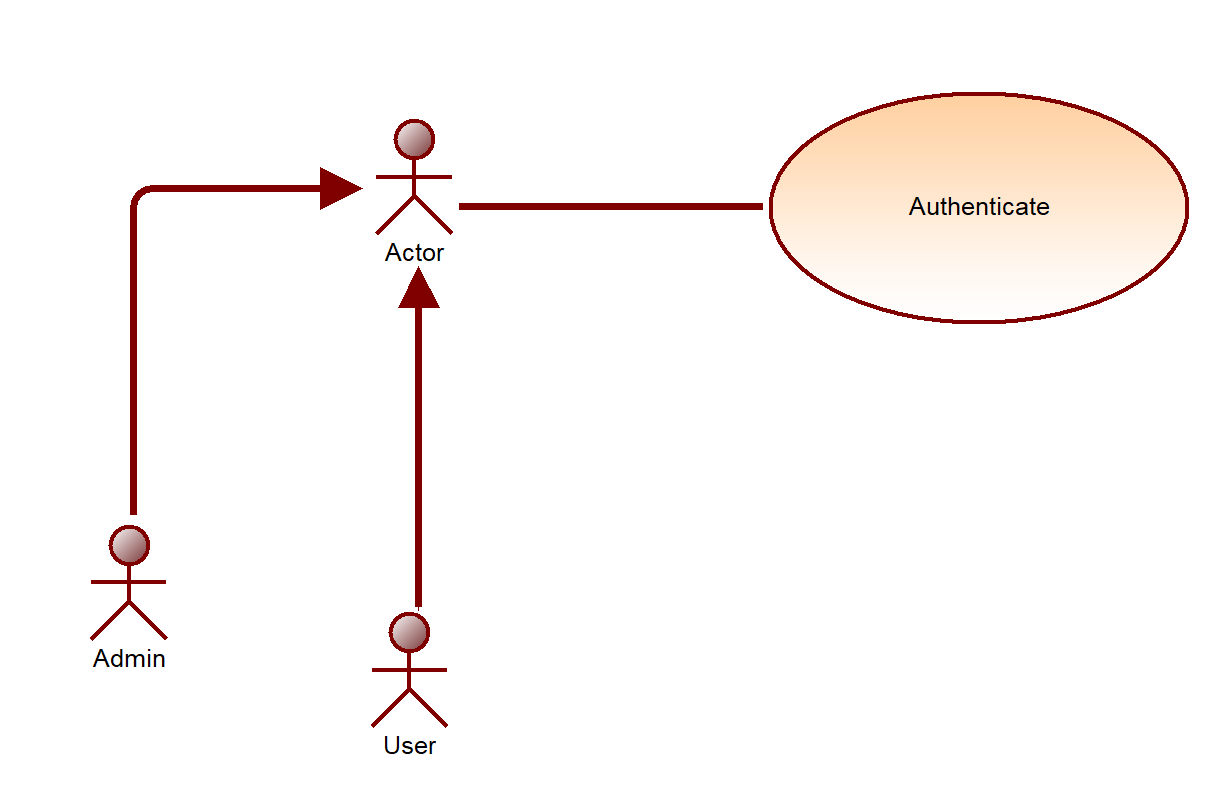
\includegraphics[width=0.3\textwidth]{Authenticate}
    \caption{use case diagram “authenticate”}
    \label{fig:design2}
\end{figure}
\newpage
\noindent
CHAPTER 2.  Sprint 0 \\
\underline{\hspace{\textwidth}} \vspace{0.2cm}\\

\begin{table}[h]
    \centering
    \begin{tabularx}{\textwidth}{X|X}
        \toprule
        Use Case Scenario & Authenticate \\
        \midrule
        Actors & Administrator / User \\
        \midrule
        Pre-Conditions & The User must have an account \\
        \midrule
        Post-Conditions & Authenticate \\
        \midrule
        Describe Main Scenario &  \begin{itemize}[label=$\bullet$]
            \item The user types the email and password
            \item The user clicks on the login button
            \item The system verifies the email and password If they are correct then :
            \item The system redirects the user to the home page 
            \item If not then :
	  \item The system displays an alert to indicate the error
        \end{itemize} \\
        \midrule
        Scenarios &  Give Opinions, View recipes \\
        \bottomrule
    \end{tabularx}
    \caption{Detailed description of the actors}
    \label{tab:actors_roles}
\end{table}
\newpage
\noindent
CHAPTER 2.  Sprint 0 \\
\underline{\hspace{\textwidth}} \vspace{0.2cm}\\
{\large \textbf{Refinement of the user story ”Add Recipes”}
\begin{figure}[htbp]
    \centering
    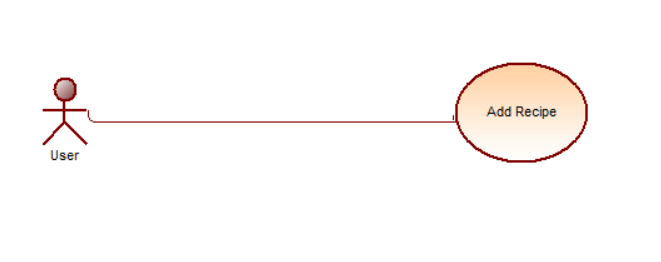
\includegraphics[width=0.5\textwidth]{Addrecipee}
    \caption{use case diagram “Add Recipes”}
    \label{fig:design2}
\end{figure}
\begin{table}[h]
    \centering
    \begin{tabularx}{\textwidth}{X|X}
        \toprule
        Use Case Scenario & Add Recipes \\
        \midrule
        Actors & User \\
        \midrule
        Pre-Conditions & The user must be authenticated \\
        \midrule
        Post-Conditions & Recipe added  \\
        \midrule
        Describe Main Scenario &  \begin{itemize}[label=$\bullet$]
            \item The user clicks on the "+"(Add) button
            \item The system displays the form interface
            \item The user fills out the form and clicks on "Add"
        \end{itemize} \\
        \bottomrule
    \end{tabularx}
    \caption{Detailed description of the actors}
    \label{tab:actors_roles}
\end{table}



\newpage
\noindent
CHAPTER 2.  Sprint 0 \\
\underline{\hspace{\textwidth}} \vspace{0.2cm}\\
{\large \textbf{Refinement of the user story ”Manage Categories”}
\begin{figure}[htbp]
    \centering
    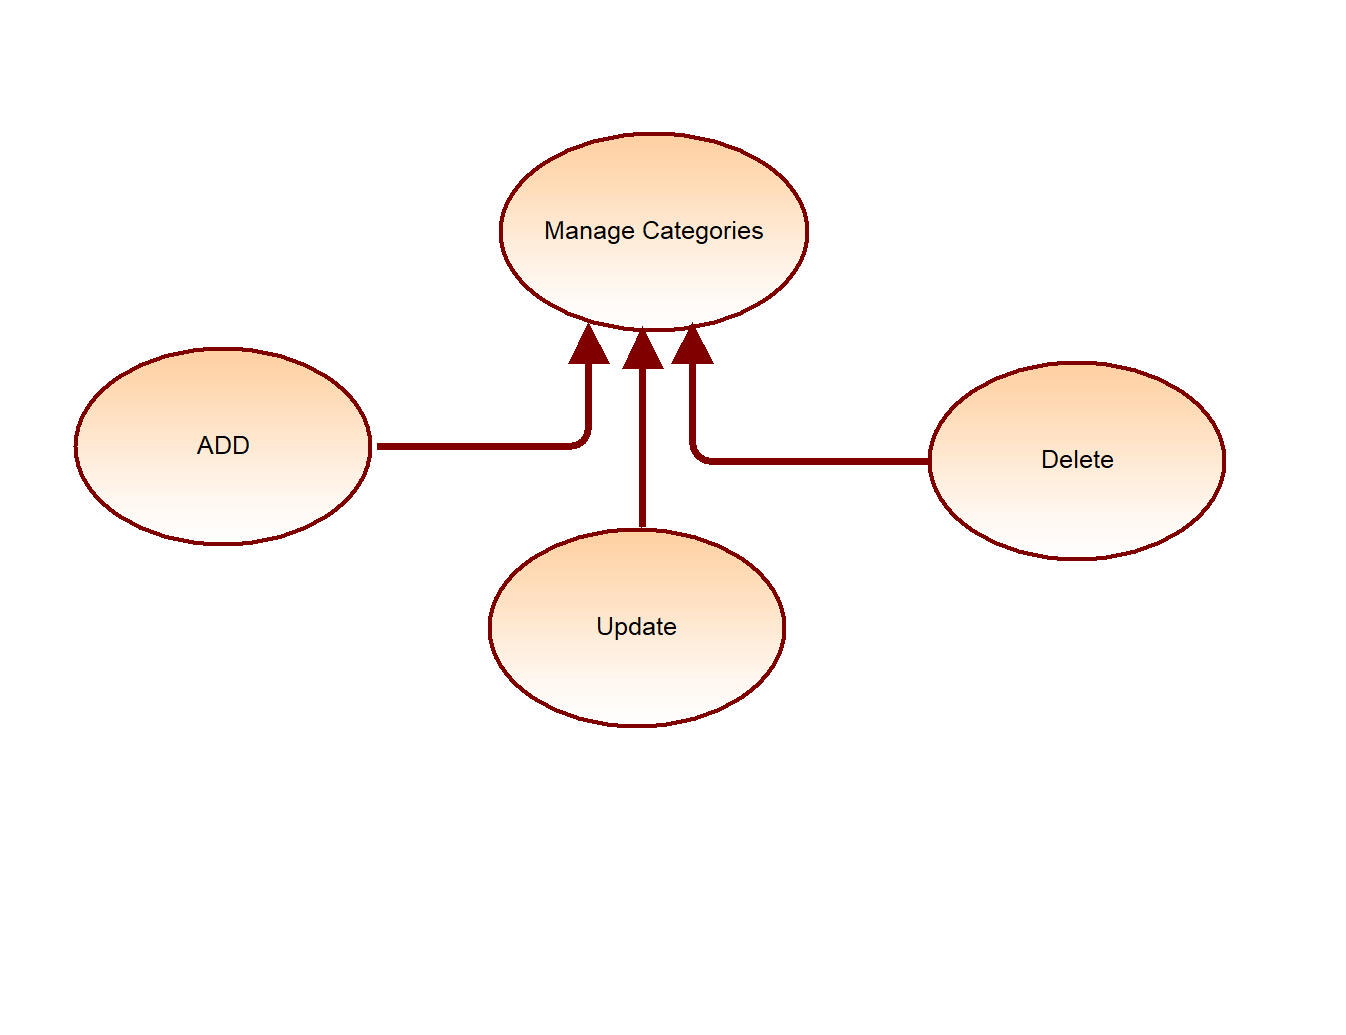
\includegraphics[width=0.5\textwidth]{Manage}
    \caption{use case diagram “Manage Categories”}
    \label{fig:design2}
\end{figure}
\begin{table}[h]
    \centering
    \begin{tabularx}{\textwidth}{X|X}
        \toprule
        Use Case Scenario & Manage Categories \\
        \midrule
        Actors & Admin \\
        \midrule
        Pre-Conditions & \begin{itemize}[label=$\bullet$]
            \item The administrator must be authenticated
            \item The system in operation
        \end{itemize} \\
        \midrule
        Post-Conditions & Categories Managed  \\
        \midrule
        Describe Main Scenario &  \begin{itemize}[label=$\bullet$]
            \item The system displays the interface
            \item The admin chooses the operation
            \item The system displays the interface according to the choice of the admin
        \end{itemize} \\
        \bottomrule
    \end{tabularx}
    \caption{Detailed description of the actors}
    \label{tab:actors_roles}
\end{table}
%-------------------------------------------------------------------------------------------------------------
\newpage
\noindent
CHAPTER 2.  Sprint 0 \\
\underline{\hspace{\textwidth}} \vspace{0.2cm}\\
\\{\Large \textbf{2.4\hspace{1em}Conception of Sprint 0}}\vspace{0.2cm}

The following figure represents the sequence diagram of Authenticate.\\

\begin{figure}[htbp]
    \centering
    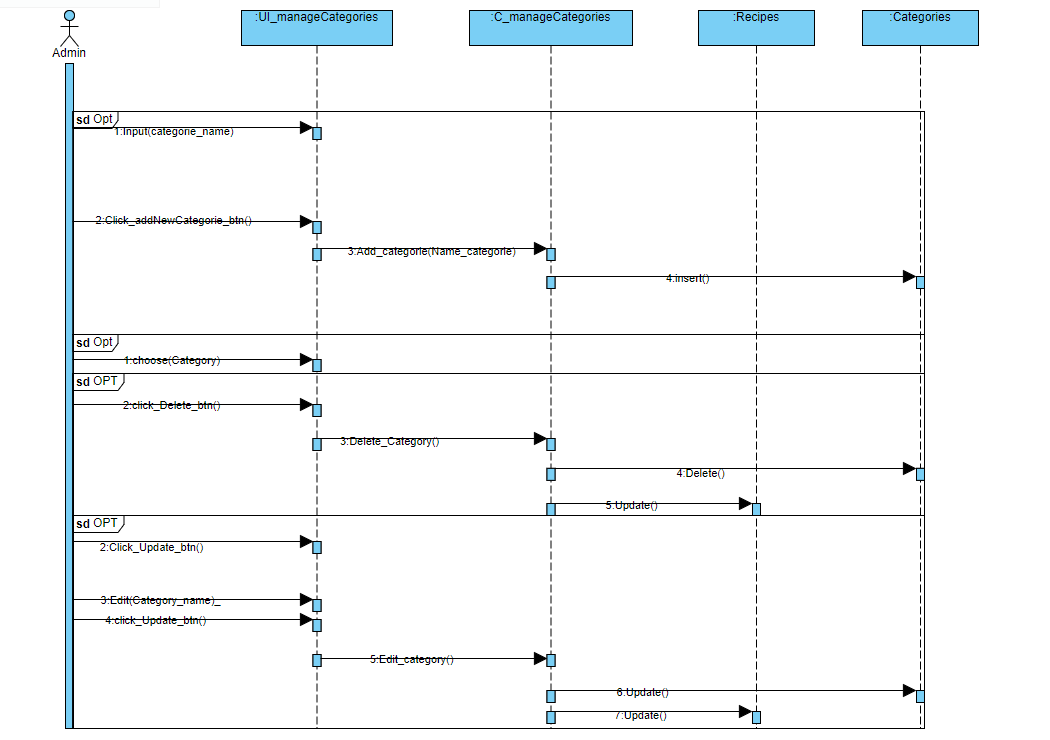
\includegraphics[width=0.9\textwidth]{autdia}
    \caption{use case diagram “View recipes”}
    \label{fig:design2}
\end{figure}
%--------------------------------------------------------------------------------------------------------------------
\newpage
\noindent
CHAPTER 2.  Sprint 0 \\
\underline{\hspace{\textwidth}} \vspace{0.2cm}\\
The following figure represents the sequence diagram of Add recipes.\\

\begin{figure}[htbp]
    \centering
    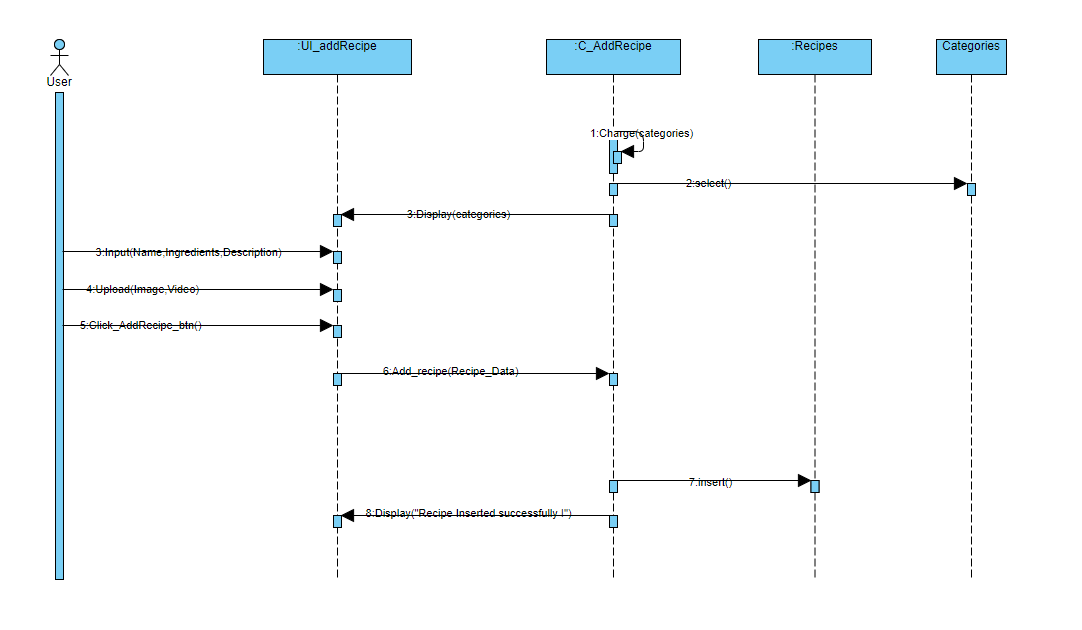
\includegraphics[width=0.9\textwidth]{adddia}
    \caption{use case diagram “View recipes”}
    \label{fig:design2}
\end{figure}
%------------------------------------------------------------------------------------------------------------------------------
\newpage
\noindent
CHAPTER 2.  Sprint 0 \\
\underline{\hspace{\textwidth}} \vspace{0.2cm}\\
The following figure represents the sequence diagram of Manage categories.\\

\begin{figure}[htbp]
    \centering
    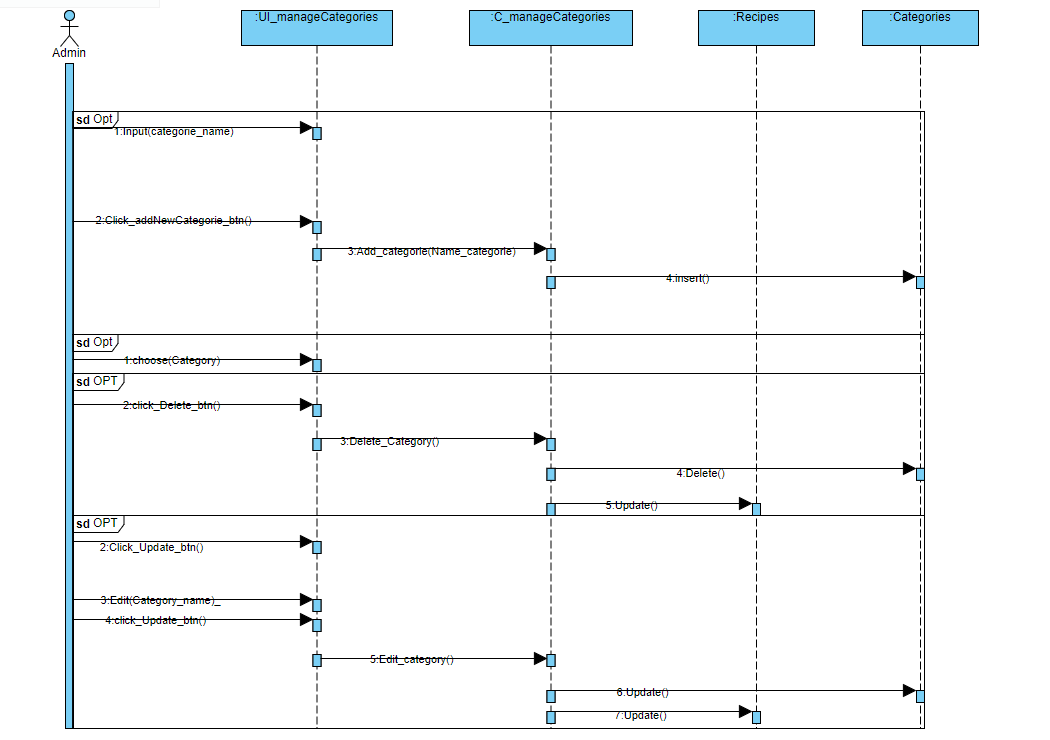
\includegraphics[width=0.9\textwidth]{mandia}
    \caption{use case diagram “View recipes”}
    \label{fig:design2}
\end{figure}
%------------------------------------------------------------------------------------------------------------------------------
\newpage
\noindent
CHAPTER 2.  Sprint 0 \\
\underline{\hspace{\textwidth}} \vspace{0.2cm}\\
 {\Large \textbf{2.5\hspace{1em}Realization of Sprint 0}}\vspace{0.2cm}\\

\textbf{Realization of the user story “authenticate”}\\
the following figure displays the login interface used by all users. It includes two fields for entering their credentials. Once authenticated, users can access role-specific dashboards.\\

\begin{figure}[htbp]
    \centering
    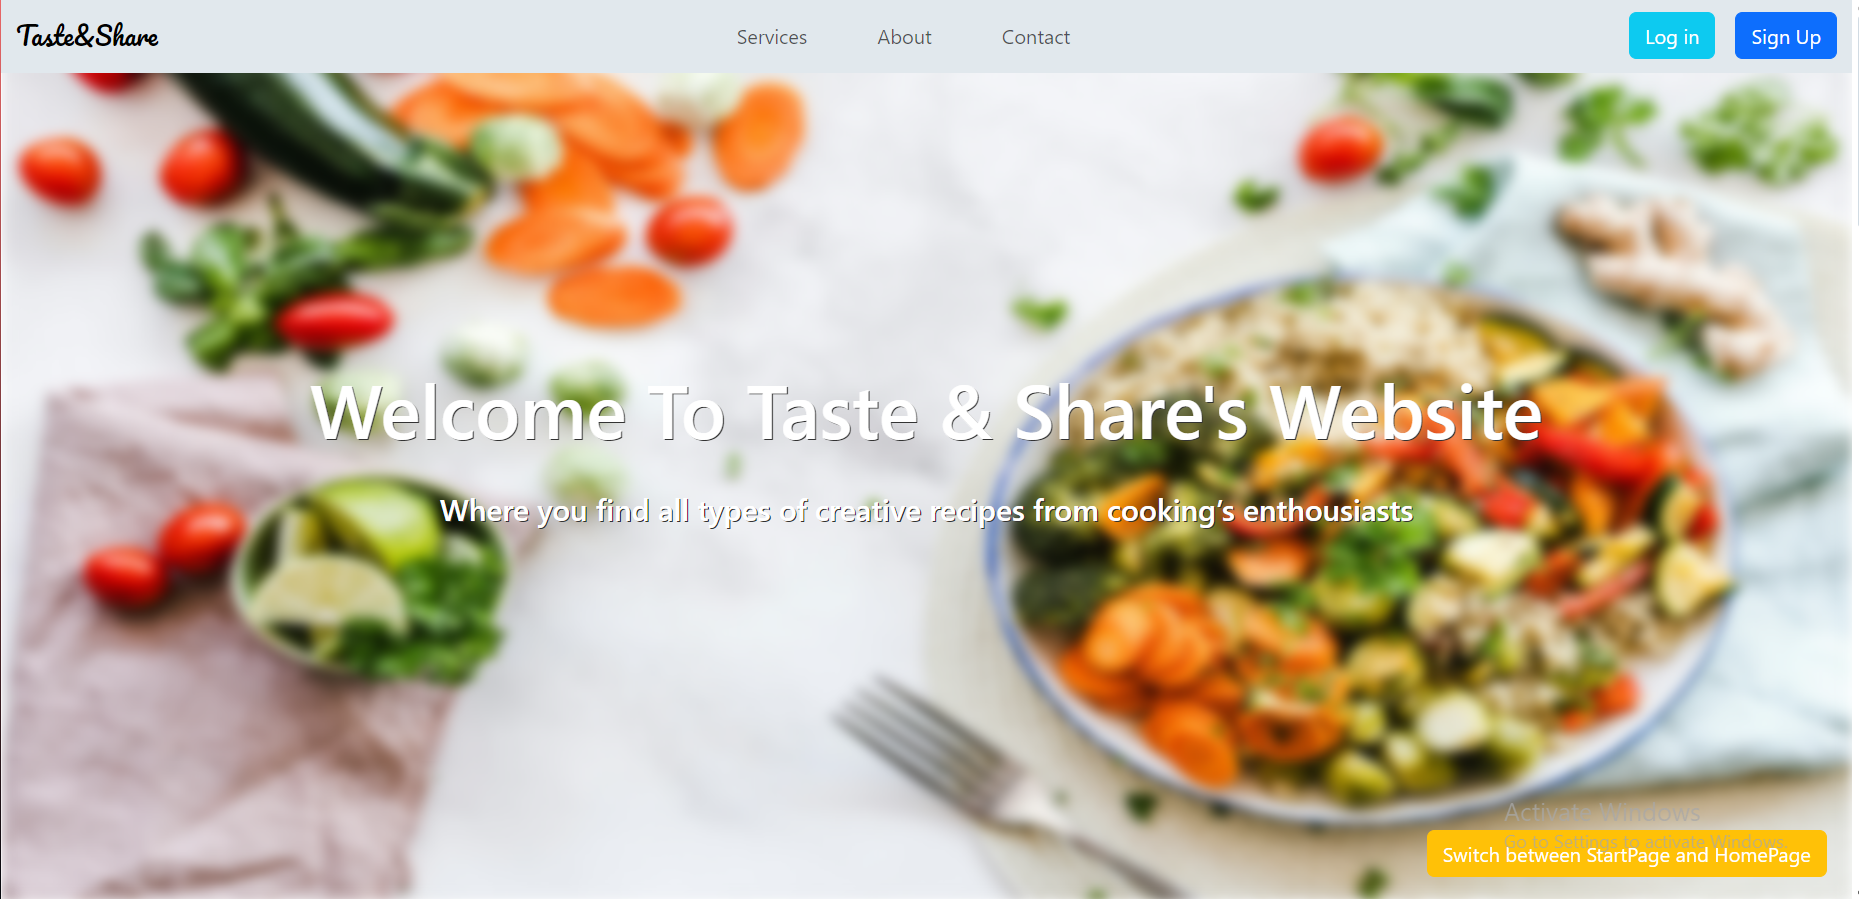
\includegraphics[width=0.5\textwidth]{wlcm} 
    \vspace{0.5cm}
    \textbf{Figure:} Home Page \\
    The user interacts with this interface to sign in or log in. A sign-up form will pop up when the user presses the "Sign Up" button.
\end{figure}

\begin{figure}[htbp]
    \centering
    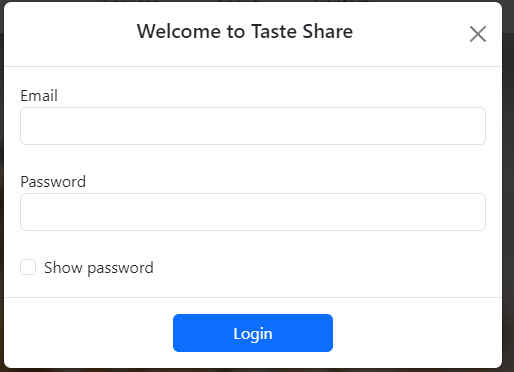
\includegraphics[width=0.5\textwidth]{logtaste}
    \caption{Authenticate Interface}
    \label{fig:design2}
\end{figure}
%--------------------------------------------------------------------------------------------------------------------------------
\newpage
\noindent
CHAPTER 2.  Sprint 0 \\
\underline{\hspace{\textwidth}} \vspace{0.2cm}\\

\textbf{Realization of the user story “Add Recipes”}\\
The image exhibits the Add Recipes interface accessible to all users, presenting six fields for inputting Recipe information. Upon completion, users can simply click 'Add Recipe' to publish it.\\

\begin{figure}[htbp]
    \centering
    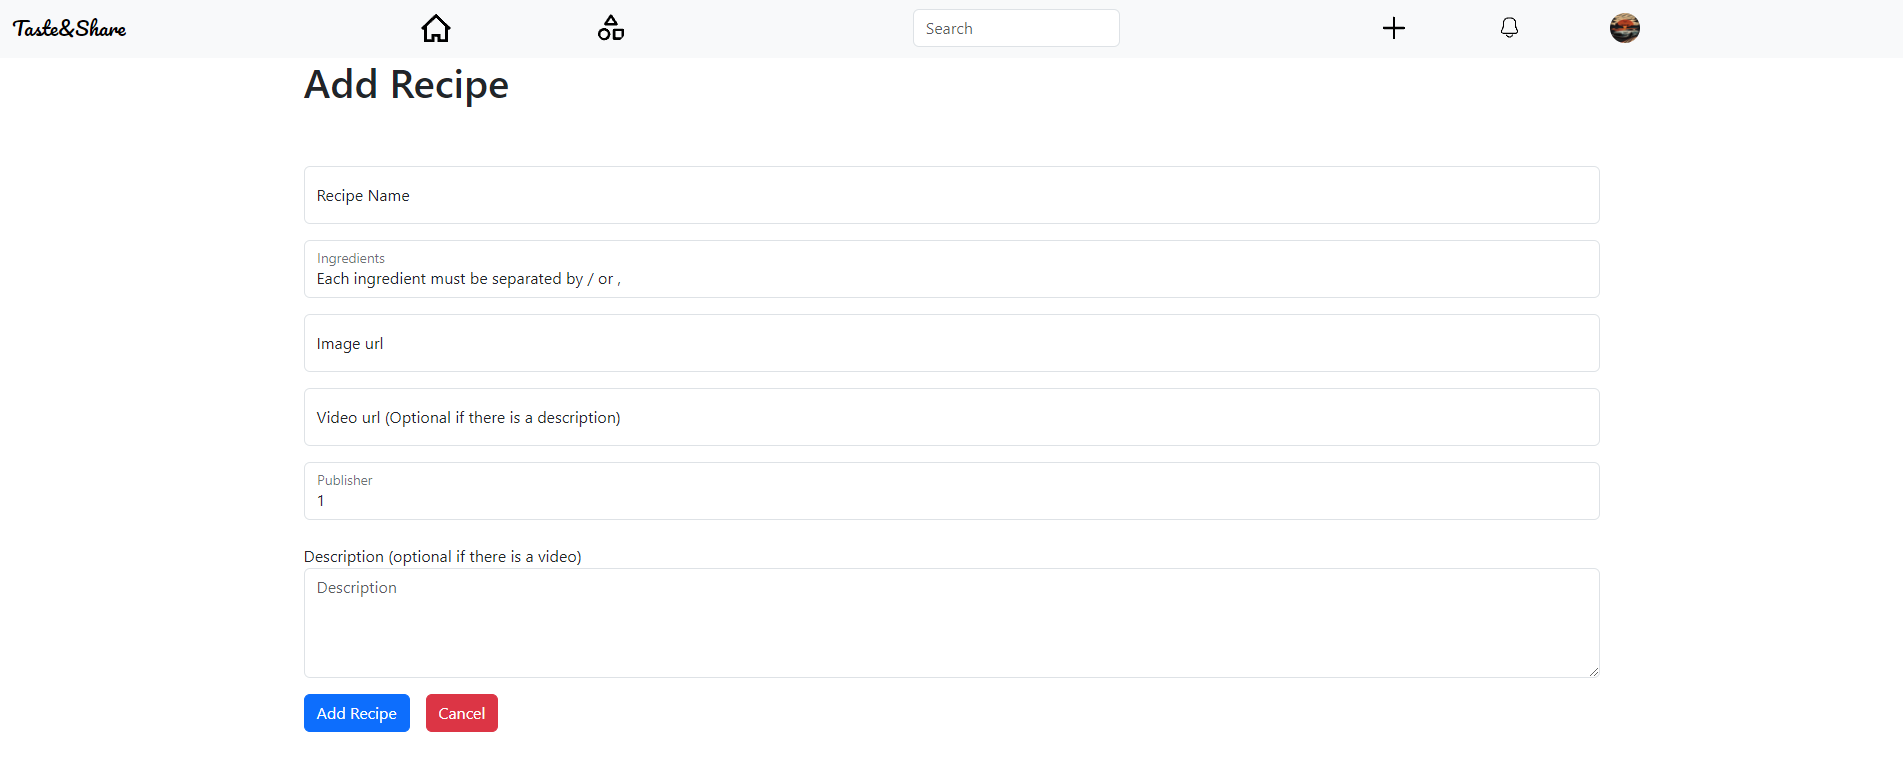
\includegraphics[width=1\textwidth]{addpic}
    \caption{Add Recipes Interface}
    \label{fig:design2}
\end{figure}
%----------------------------------------------------------------------------------------------------------------------------------------------
\newpage
\noindent
CHAPTER 2.  Sprint 0 \\
\underline{\hspace{\textwidth}} \vspace{0.2cm}\\

\textbf{Realization of the user story “Manage Categories”}\\
The depicted figure showcases the admin's interface for managing categories, allowing him to add, edit, or delete categories as needed.\\

\begin{figure}[htbp]
    \centering
    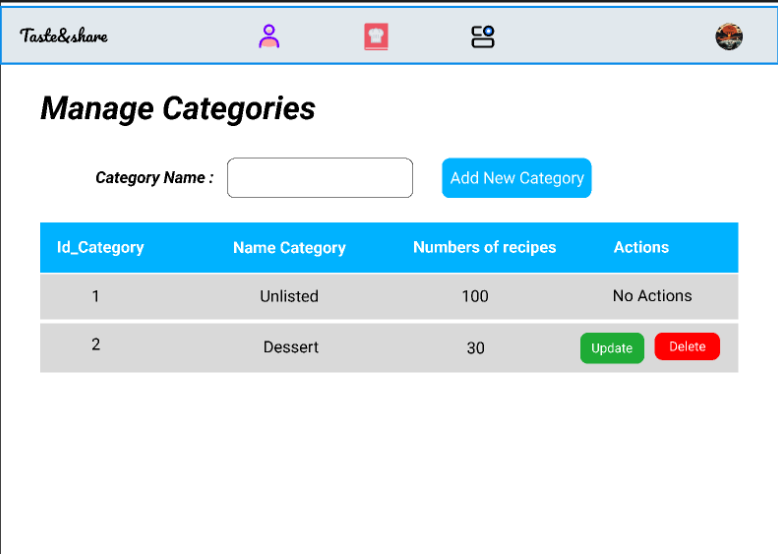
\includegraphics[width=1\textwidth]{mapic}
    \caption{Manage categories Interface}
    \label{fig:design2}
\end{figure}
 {\Large \textbf{2.6\hspace{1em}Conclusion}}\vspace{0.2cm}\\
empty

%------------------------------------------------------------------------------------------------------------------------------------------------------
\newpage
\section*{\Huge CHAPTER 3\vspace{0.5cm}\\Sprint 1}
\vspace{1.5cm}

{\Large \textbf{3.1\hspace{1em}Introduction}}\vspace{0.2cm}
\\empty
\\{\Large \textbf{3.2\hspace{1em}Identification of Sprint 1 Backlog}}\vspace{0.2cm}
\\The following table contains the backlog elements that are realised during the sprint 1 :
\begin{table}[h]
    \centering
    \begin{tabularx}{\textwidth}{lX@{\hspace{1em}}c@{\hspace{7em}}c} 
        \toprule
        \textbf{\color{blue!70} User Story} & \textbf{\color{blue!70} Priority} & \textbf{\color{blue!70} Sprint} & \textbf{\color{blue!70} Estimation} \\ 
        \midrule

         As a User I can view recipes & 2 & 1& Medium \\
        \midrule
        As a user, I can contact other users & 2 & 1 & High \\
        \midrule
        As an admin, I can manage users & 2 & 1 & High \\
        \bottomrule
    \end{tabularx}
\end{table}


















%-------------------------------------------------------------------------------------------------------------------------
\newpage
\noindent
CHAPTER 3.  Sprint 1 \\
\underline{\hspace{\textwidth}} \vspace{0.2cm}\\
\\{\Large \textbf{3.3\hspace{1em}Refinement of sprint 1}}\vspace{0.2cm}
\\In this section, we examine various use-case scenarios for the sprint 1.\\
{\large \textbf{Refinement of the user story ”View recipes ”}
\begin{figure}[htbp]
    \centering
    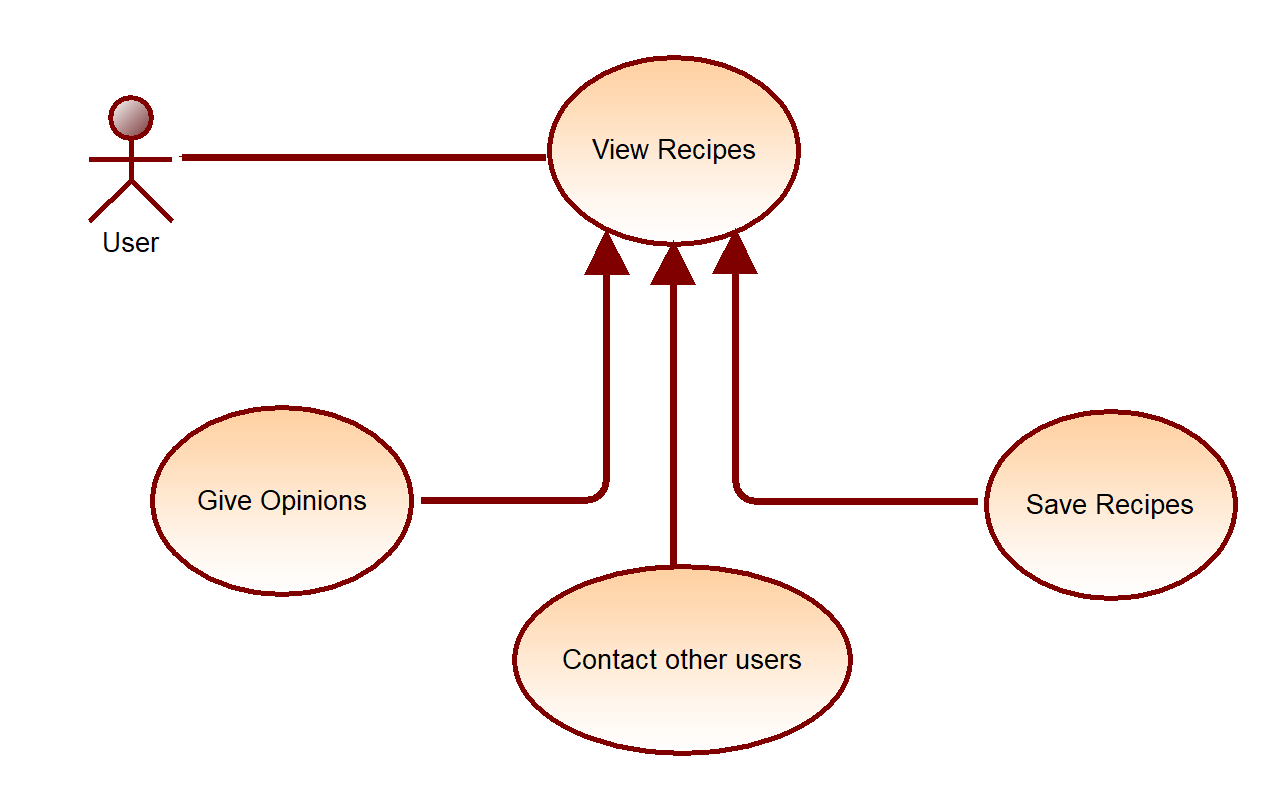
\includegraphics[width=0.5\textwidth]{view}
    \caption{use case diagram “View recipes”}
    \label{fig:design2}
\end{figure}
\begin{table}[h]
    \centering
    \begin{tabularx}{\textwidth}{X|X}
        \toprule
        Use Case Scenario & View recipes  \\
        \midrule
        Actors & User \\
        \midrule
        Pre-Conditions &  The user must be authenticated \\
        \midrule
        Post-Conditions & Recipe accessed  \\
        \midrule
        Describe Main Scenario &  
        \begin{itemize}[label=$\bullet$]
            \item The user clicks on the recipe
            \item The system displays the recipe interface
            \item The user selects their preferred format for viewing the recipe: either video or text 
        \end{itemize} \\
        \bottomrule
    \end{tabularx}
    \caption{Detailed description of the actors}
    \label{tab:actors_roles}
\end{table}




%-------------------------------------------------------------------------------------------------------------------------
\newpage
\noindent
CHAPTER 3.  Sprint 1 \\
\underline{\hspace{\textwidth}} \vspace{0.2cm}\\
{\large \textbf{Refinement of the user story ”Give Opinions”}
\begin{figure}[htbp]
    \centering
    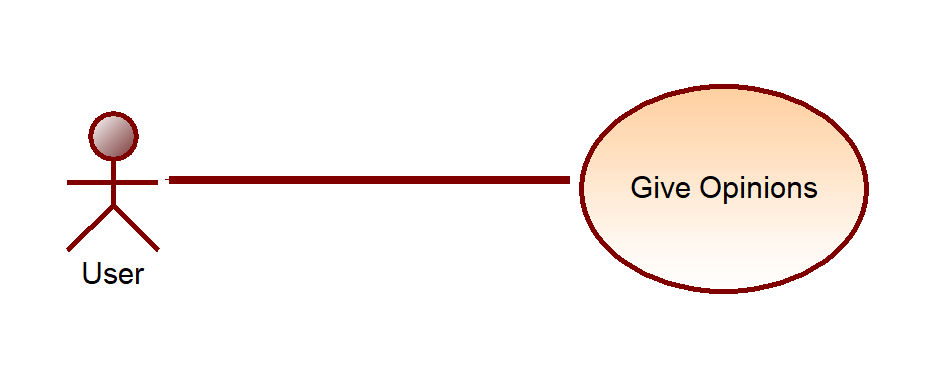
\includegraphics[width=0.5\textwidth]{opin}
    \caption{use case diagram “Give Opinions”}
    \label{fig:design2}
\end{figure}
\begin{table}[h]
    \centering
    \begin{tabularx}{\textwidth}{X|X}
        \toprule
        Use Case Scenario & Give Opinions \\
        \midrule
        Actors & User \\
        \midrule
        Pre-Conditions & \begin{itemize}[label=$\bullet$]
            \item The administrator must be authenticated
           
        \end{itemize} \\
        \midrule
        Post-Conditions & Opinion Given  \\
        \midrule
        Describe Main Scenario &  \begin{itemize}[label=$\bullet$]
            \item - The user clicks on the recipe
            \item- The system displays the recipe interface
	\item- The user reacts to the recipe with a heart and writes a comment
           
        \end{itemize} \\
        \bottomrule
    \end{tabularx}
    \caption{Detailed description of the actors}
    \label{tab:actors_roles}
\end{table}
\newpage
\noindent
CHAPTER 3.  Sprint 1 \\
\underline{\hspace{\textwidth}} \vspace{0.2cm}\\
{\large \textbf{Refinement of the user story ”Save Recipes”}
\begin{figure}[htbp]
    \centering
    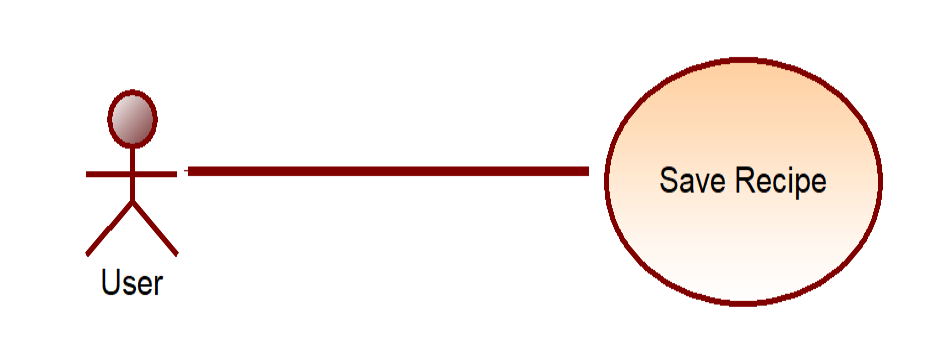
\includegraphics[width=0.5\textwidth]{save}
    \caption{use case diagram “Save Recipes”}
    \label{fig:design2}
\end{figure}
\begin{table}[h]
    \centering
    \begin{tabularx}{\textwidth}{X|X}
        \toprule
        Use Case Scenario & Save Recipes\\
        \midrule
        Actors & User \\
        \midrule
        Pre-Conditions & \begin{itemize}[label=$\bullet$]
            \item The user must be authenticated
           
        \end{itemize} \\
        \midrule
        Post-Conditions & Recipe saved  \\
        \midrule
        Describe Main Scenario &  \begin{itemize}[label=$\bullet$]
            \item - The user clicks on the save button below any recipe
            \item- The system displays a message : "Recipe saved"
	
           
        \end{itemize} \\
        \bottomrule
    \end{tabularx}
    \caption{Detailed description of the actors}
    \label{tab:actors_roles}
\end{table}






















\newpage
\noindent
CHAPTER 3.  Sprint 1 \\
\underline{\hspace{\textwidth}} \vspace{0.2cm}\\
{\large \textbf{Refinement of the user story ”Contact other users"}
\begin{figure}[htbp]
    \centering
    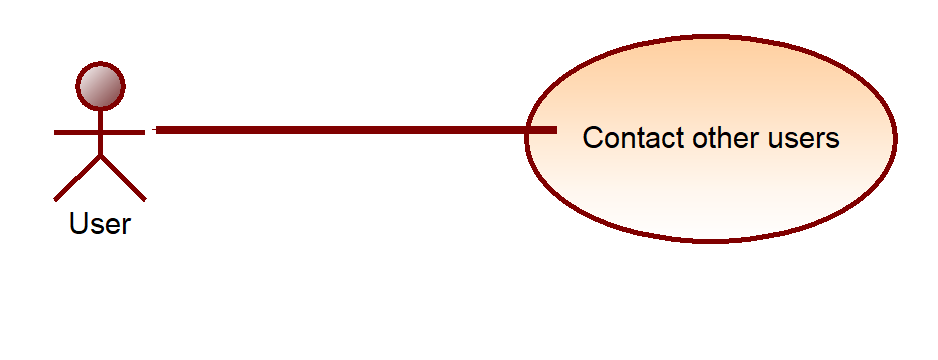
\includegraphics[width=0.5\textwidth]{conta}
    \caption{use case diagram “Contact other users”}
    \label{fig:design2}
\end{figure}
\begin{table}[h]
    \centering
    \begin{tabularx}{\textwidth}{X|X}
        \toprule
        Use Case Scenario & Contact other users \\
        \midrule
        Actors & User \\
        \midrule
        Pre-Conditions & The user must be authenticated \\
        \midrule
	 Post-Conditions & Other users contaced  \\
        \midrule
        Describe Main Scenario &  \begin{itemize}[label=$\bullet$]
            \item The user clicks on the recipe
            \item The system displays recipe
            \item The user clicks on the "Contact The Publisher" button
        \end{itemize} \\
        \bottomrule
    \end{tabularx}
    \caption{Detailed description of the actors}
    \label{tab:actors_roles}
\end{table}















\newpage
\noindent
CHAPTER 3.  Sprint 1 \\
\underline{\hspace{\textwidth}} \vspace{0.2cm}\\
{\large \textbf{Refinement of the user story ”Manage Users”}
\begin{figure}[htbp]
    \centering
    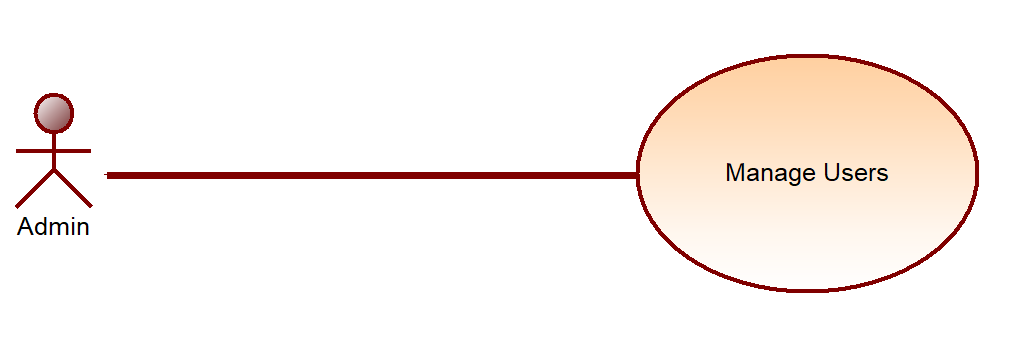
\includegraphics[width=0.5\textwidth]{muse}
    \caption{use case diagram “Manage Users”}
    \label{fig:design2}
\end{figure}
\begin{table}[h]
    \centering
    \begin{tabularx}{\textwidth}{X|X}
        \toprule
        Use Case Scenario & Manage Users \\
        \midrule
        Actors & User \\
        \midrule
        Pre-Conditions & \begin{itemize}[label=$\bullet$]
\item The user must be authenticated 
\item the system in operation
 \end{itemize} \\
        \midrule
	 Post-Conditions & Users Managed  \\
        \midrule
        Describe Main Scenario &  \begin{itemize}[label=$\bullet$]
            \item - The administrator chooses whether to add or ban users
            \item- The administrator chooses to add or remove moderators
    
        \end{itemize} \\
        \bottomrule
    \end{tabularx}
    \caption{Detailed description of the actors}
    \label{tab:actors_roles}
\end{table}
%---------------------------------------------------------------------------------------------------------------conception de sprint 1

























%%---------------------------------------------------------------------------------------------------------------------------------------------------------
\newpage
\noindent
CHAPTER 3.  Sprint 1 \\
\underline{\hspace{\textwidth}} \vspace{0.2cm}

{\Large \textbf{3.5\hspace{1em}Realization of Sprint 1}}\vspace{0.2cm}
\\\textbf{Realization of the user story “View Recipes”}\\
The depicted figure showcases the View Recipes interface, empowering users to seamlessly access recipes, save their favorites, rate dishes, and connect with other users for culinary insights.\\
\begin{figure}[htbp]
    \centering
    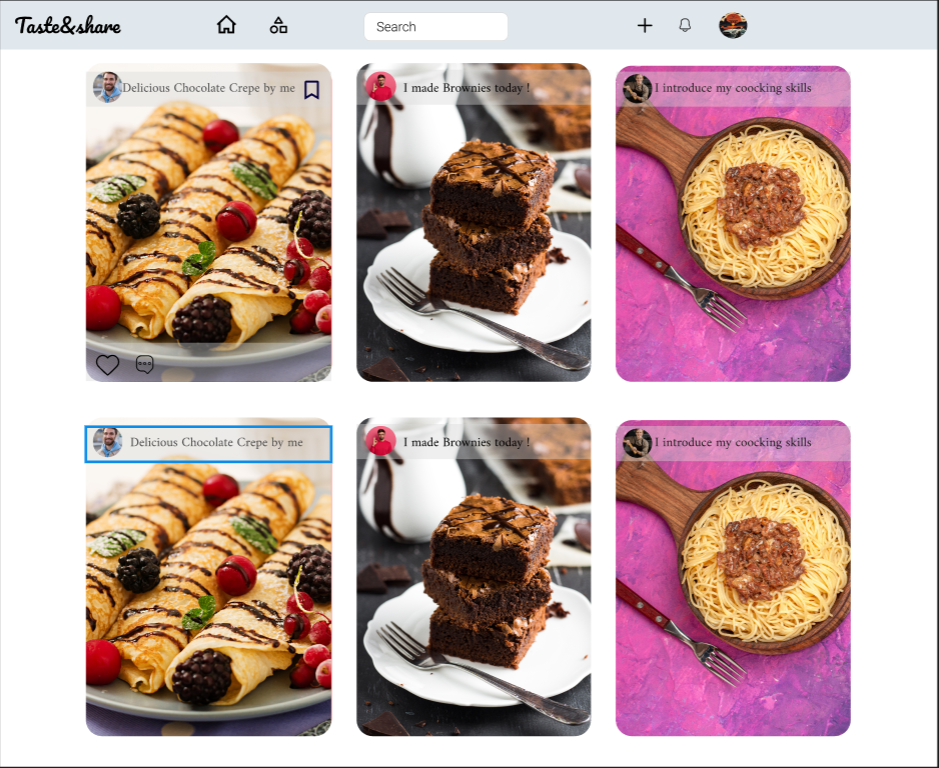
\includegraphics[width=0.5\textwidth]{ViewRecipes} 
    \vspace{0.5cm}
    
    \textbf{Figure:} View Recipes Page \\
    The user can view other users' recipes using this interface.
\end{figure}
%--------------------------------------------------------------------------------------------
\newpage
\noindent
CHAPTER 3.  Sprint 1 \\
\underline{\hspace{\textwidth}} \vspace{0.2cm}

\begin{figure}[htbp]
    \centering
    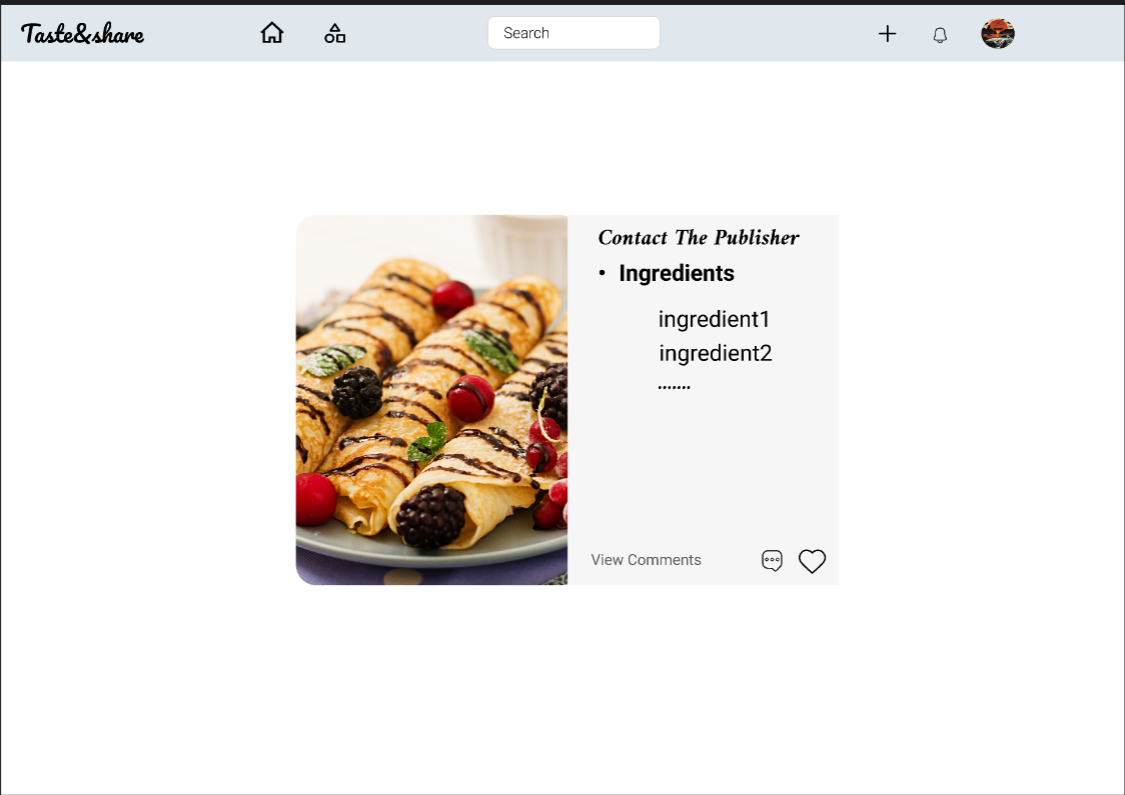
\includegraphics[width=0.5\textwidth]{ViewRecipes2} 
    \vspace{0.5cm}
    
    \textbf{Figure:} View Recipes Page (Detail) \\
    When the user clicks on a recipe, the website will display the recipe details, including any available video. The user can interact with the recipe by saving it, liking it, commenting on it, viewing ingredients, or contacting the publisher.
\end{figure}

\begin{figure}[htbp]
    \centering
    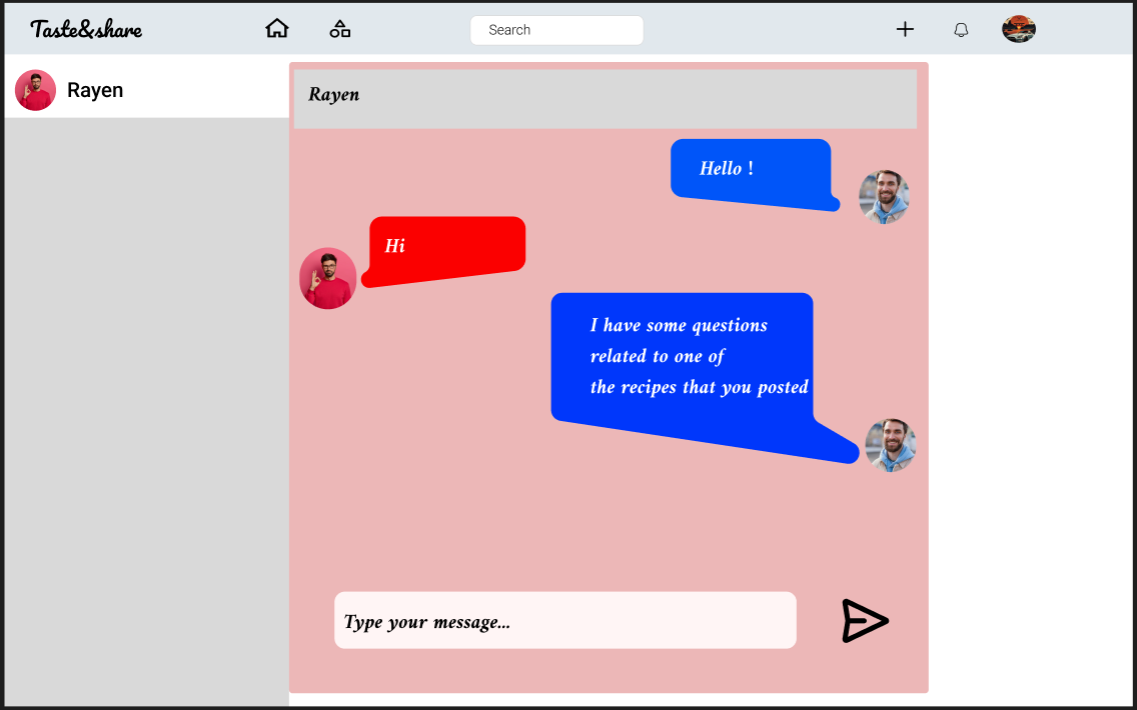
\includegraphics[width=0.5\textwidth]{Contact} 
    \vspace{0.5cm}
    
    \textbf{Figure:} Contact Publisher Interface \\
    When the user clicks on the "Contact the Publisher" button, a small chat room will be created between the user and the publisher.
\end{figure}
%--------------------------------------------------------------------------------------------------------------------------------------------
\newpage
\noindent
CHAPTER 3.  Sprint 1 \\
\underline{\hspace{\textwidth}} \vspace{0.2cm}
\\\textbf{Realization of the user story “Manage Users”}\\
The depicted figure showcases the Manage Users interface, granting the admin comprehensive control over user management tasks such as updating, deleting, and overseeing user accounts. Additionally, the admin possesses the capability to manage and remove comments efficiently.\\
\begin{figure}[htbp]
    \centering
    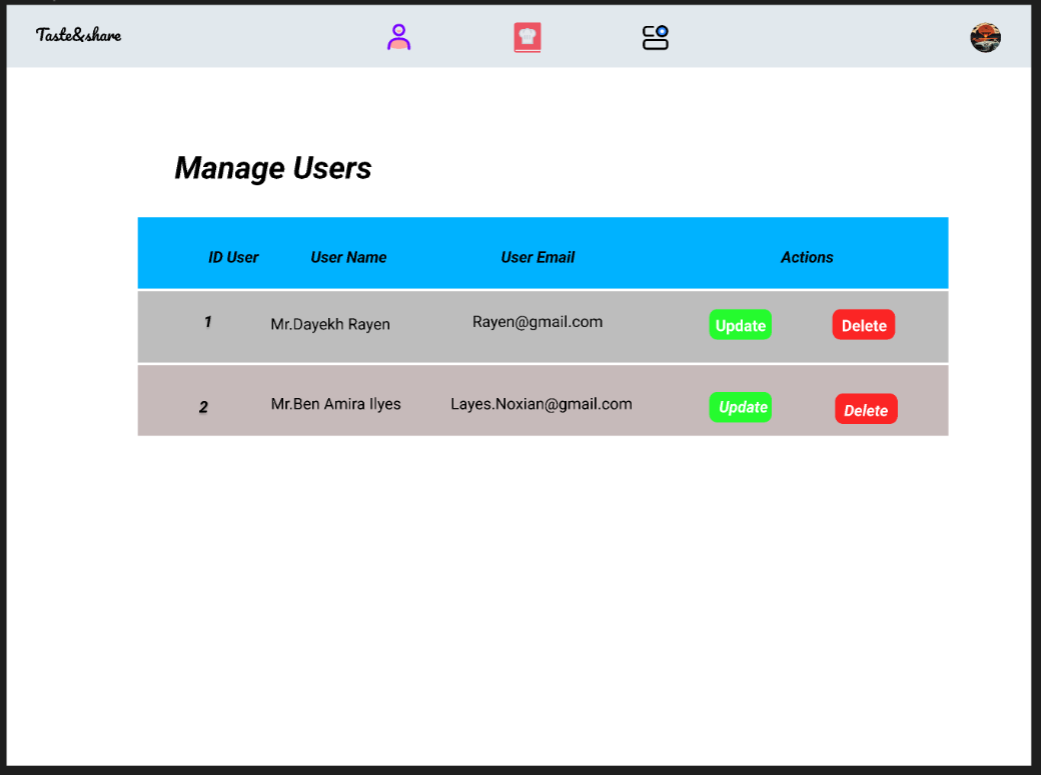
\includegraphics[width=0.5\textwidth]{ManageUser} 
    \vspace{0.5cm}
    
    \textbf{Figure:} Manage Users Interface \\
    The admin can manage all users, including updating user information or deleting users. When the admin clicks the "Update" button, another page will open to update user information.
\end{figure}

\begin{figure}[htbp]
    \centering
    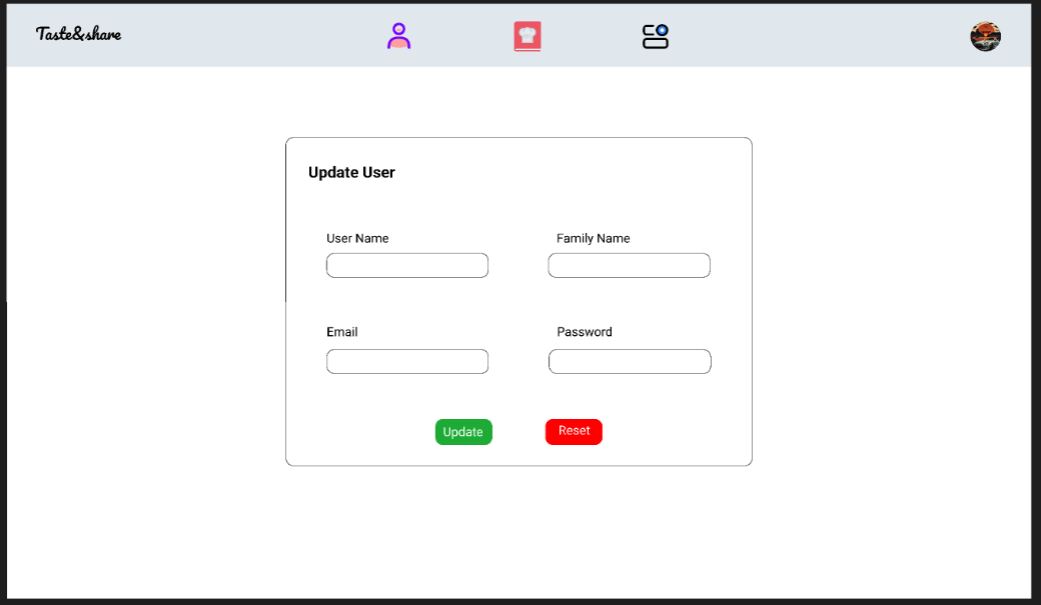
\includegraphics[width=0.5\textwidth]{UpdateUser} 
    \vspace{0.5cm}
    
    \textbf{Figure:} Update User Page \\
    The admin can update user information using this interface.
\end{figure}
\newpage
\noindent
CHAPTER 3.  Sprint 1 \\
\underline{\hspace{\textwidth}} \vspace{0.2cm}
\begin{figure}[htbp]
    \centering
    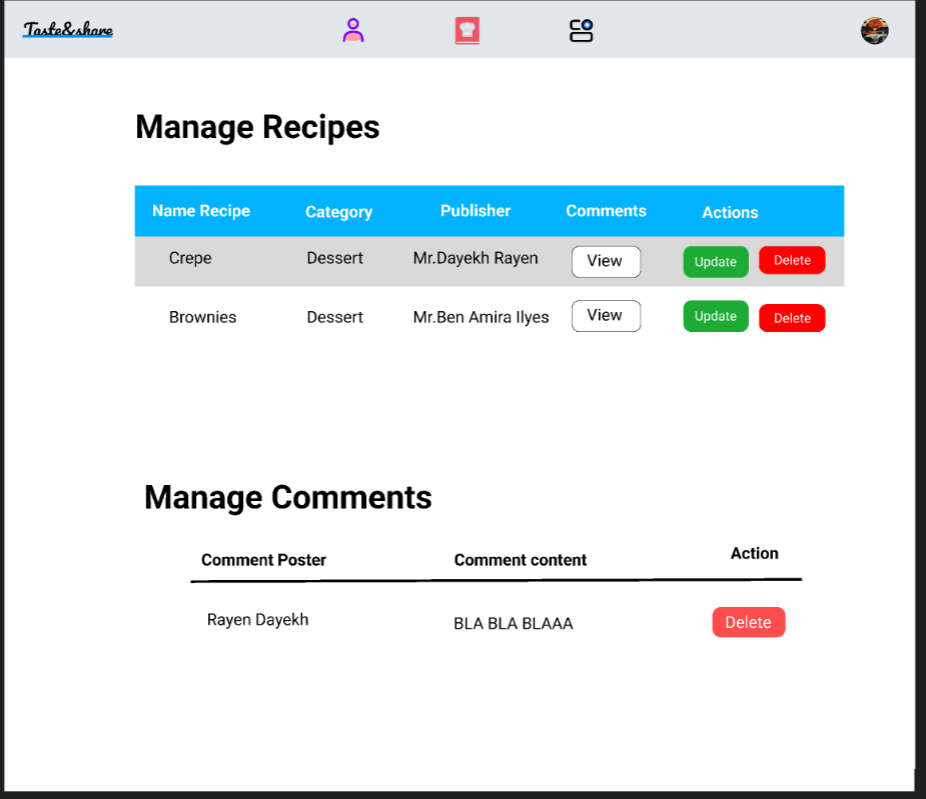
\includegraphics[width=0.5\textwidth]{ManageRecipes} 
    \vspace{0.5cm}
    
    \textbf{Figure:} Manage Recipes Interface \\
    The admin can manage recipes using this interface. Clicking the "View" button will display all comments on that recipe, allowing the admin to delete them. Clicking the "Update" button will open another page to update the recipe name and category.
\end{figure}\\
{\Large \textbf{3.6\hspace{1em}Conclusion}}\vspace{0.2cm}\\
empty
\newpage
\section*{ \Huge General Conclusion}\vspace{0.5cm} 
\setstretch{1.5}
empty
\newpage
{\LARGE \textbf{\hspace{1em}Bibliography}}\vspace{0.5cm}

\begin{itemize}
    \item [1.] \url{https://code.visualstudio.com/docs}
    \item [2.] \url{https://www.php.net/manual/fr/intro-whatis.php}
    \item [3.] \url{https://angular.io/guide/what-is-angular}
    \item [4.] \url{https://www.oracle.com/mysql/what-is-mysql/}
    \item [5.] \url{https://www.apachefriends.org/fr/about.html}
    \item [6.] \url{https://www.powerdesigner.biz/}
\end{itemize}



\end{document}


